%% Slides for ".NET Programming" by Chunyu Wang <chunyu@hit.edu.cn> %%

\section{C\# 3.0/4.0}

\begin{frame}[fragile]
\frametitle{隐含类型局部变量(\textit{Implicitly typed local variable})}

\begin{itemize}
\item 关键字\texttt{var} 可用于声明局部变量
\item 具体类型由编译器根据初始化表达式推断
\begin{lstlisting}
  var i = 5;
  var s = "Hello";
  var d = 1.0;
  var numbers = new int[] {1, 2, 3};
  var orders = new Dictionary<int,Order>();
\end{lstlisting}

\item 上面的声明等价于
\begin{lstlisting}
  int i = 5;
  string s = "Hello";
  double d = 1.0;
  int[] numbers = new int[] {1, 2, 3};
  Dictionary<int,Order>
      orders = new Dictionary<int,Order>();
\end{lstlisting}
\end{itemize}
\end{frame}

\begin{frame}[fragile]
\frametitle{隐含类型局部变量(2)}
\begin{itemize}
\item 隐式类型必须初始化,用于编译器推断类型
\item 初始化时,值不能是\texttt{null}
\item 如下的几种声明,编译器无法推断类型
\begin{lstlisting}[escapeinside=<>]
var x;                // <错误,没有初始化>
var y = {1, 2, 3};    // <错误,没有数组声明>
var z = null;         // <错误,null 无法推断类型>
\end{lstlisting}

\item 数组的隐含类型可以再简化
\begin{lstlisting}
var a = new[] { "hello", null, " world" }; //<string>[]
var b = new[] { new[] {1,2,3,4},
                new[] {5,6,7,8}         }; //<int>[][]

var x = new[] { 1, "one", 2, "two" };      //<Error>
\end{lstlisting}
\end{itemize}
\end{frame}

\begin{frame}[fragile]
\frametitle{隐含类型局部变量(3)}

关键字\texttt{var} 可用于以下情况
\begin{itemize}
\item 局部变量
\item 在\texttt{for} 的初始化语句中
\begin{lstlisting}
for(var x = 1; x < 10; x++) { ... }
\end{lstlisting}
\item 在\texttt{foreach} 的初始化语句中
\begin{lstlisting}
foreach(var item in list){...}
\end{lstlisting}
\item 在\texttt{using} 语句中
\begin{lstlisting}
using (var f = new StreamReader("...")) {...}
\end{lstlisting}
\end{itemize}
\end{frame}

% \begin{frame}[fragile]
% \frametitle{隐含类型数组(\textit{Implicitly typed arrays})}
% \begin{itemize}
% \item 由编译器推断数组类型
% \end{itemize}
% \begin{lstlisting}[escapeinside=<>]
% var a = new[] { 1, 10, 100, 1000 };       // <int>[]
% var b = new[] { 1, 1.5, 2, 2.5 };         // <double>[]
% var c = new[] { "hello", null, "world" }; // <string>[]
% var d = new[] { 1, "one", 2, "two" };     // <Error>
% \end{lstlisting}
% \end{frame}

\begin{frame}[fragile]
\frametitle{扩展方法(\textit{Extension Method})}
\begin{block}{\textit{Extension Methods}}
\CJKindent 定义在静态类中的特殊方法,可以在不改变现有代码的情况下,扩展为已有类型的实例方法。
\end{block}

\begin{itemize}
\item 通过编译技术,将实例方法转换为静态方法
\item 必须在静态类中实现,且不能是嵌套类或泛型类
\item 该方法的第一个参数必须有\texttt{this} 修饰
\end{itemize}

\lstset{emph={this}}
\begin{lstlisting}
public static class Extensions{
  public static void Foo(this string s) { ... }
}
...
  string s = "Hello,World";
  s.Foo();
\end{lstlisting}
\end{frame}


\begin{frame}[fragile]
\frametitle{扩展方法的示例}
\begin{itemize}
\item 为\texttt{int} 类型添加方法 \texttt{Square()}
\end{itemize}
\lstset{emph={this,static}}
\lstset{emph={[2]Square}}
\begin{lstlisting}
class Program
{
    static void Main(string[] args)
    {
        int i = 6;
        Console.WriteLine(i.Square());
        // i.Square().Square();
    }
}
static class Extensions
{
    public static int Square(this int i)
    {
        return i * i;
    }
}

\end{lstlisting}
\end{frame}

\begin{frame}[fragile]
\frametitle{扩展方法的示例(续)}

\begin{itemize}
\item 编译之后的IL 代码
\end{itemize}
\lstset{emph={[2]CSharp,Extensions,Square}}
\begin{lstlisting}
.method private hidebysig
          static void Main(string[] args) cil managed
{
  .entrypoint
  // Code size 16 (0x10)
  .maxstack  1
  .locals init ([0] int32 i)
  IL_0000: nop
  IL_0001: ldc.i4.6
  IL_0002: stloc.0
  IL_0003: ldloc.0
  IL_0004: call int32 CSharp.Extensions::Square(int32)
  IL_0009: call void [mscorlib]System.Console::WriteLine(int32)
  IL_000e: nop
  IL_000f: ret
} // end of method Program::Main
\end{lstlisting}
\end{frame}


\begin{frame}[fragile]
\frametitle{扩展方法的示例(续)}
\begin{itemize}
\item 相当于静态类函数在对象上的调用
\end{itemize}
\lstset{emph={[2]Square}}
\begin{lstlisting}
class Program
{
    static void Main(string[] args)
    {
        int i = 6;
        Console.WriteLine(Extensions.Square(i));
        // Extensions.Square(Extensions.Square(i))
    }
}
static class Extensions
{
    public static int Square(this int i)
    {
        return i * i;
    }
}

\end{lstlisting}
\end{frame}


\begin{frame}[fragile]
\frametitle{接口的扩展函数}
\begin{itemize}
\item 对接口的扩展与对类型的相同
\item 但显然不能直接在接口上调用扩展函数
\item 只能理解为,所有实现了该接口的对象上增加了扩展函数
\end{itemize}
\lstset{emph={this}}
\lstset{emph={[2]IMath}}
\begin{lstlisting}
public interface IMath
{ int Add(int x, int y);   }
class MyCalc : IMath
{ public int Add(int x, int y)  { return x + y; } }

public static class ExtIMath
{
  public static int Subtract(this IMath itf, int x, int y)
  { return x - y; }
}
...  // in Main()
  MyCalc c = new MyCalc();
  Console.WriteLine("1 + 2 = {0}", c.Add(1, 2));
  Console.WriteLine("1 - 2 = {0}", c.Subtract(1, 2));
\end{lstlisting}
\end{frame}

\begin{frame}[fragile]
\frametitle{对象初始化器(\textit{Object initializer})}
\begin{lstlisting}
public class Point
{  int x, y;
   public int X { get { return x; } set { x = value; } }
   public int Y { get { return y; } set { y = value; } }
}
\end{lstlisting}
\begin{itemize}
\item 创建对象的同时,为对象初始化成员
\begin{lstlisting}
var a = new Point { X = 0, Y = 1 };
\end{lstlisting}
\item 等同于
\begin{lstlisting}
var a = new Point();
a.X = 0;
a.Y = 1;
\end{lstlisting}
\end{itemize}
\end{frame}

\begin{frame}[fragile]
\frametitle{自动特性(\textit{Automatic Propertie})}
\begin{itemize}
\item 未使用自动特性
\begin{lstlisting}
class Person
{ private string _Name;
  public  string  Name
  { get { return _name; }
    set { _name = value; } }
}
\end{lstlisting}
\item 使用自动特性
\begin{lstlisting}
class Person
{
  public string Name { get; set; }
}
\end{lstlisting}
\item 在创建特性的同时,自动创建私有字段
\item “私有字段$+$公有特性”可以为对象提供良好的封装性。
\end{itemize}
\end{frame}

\begin{frame}[fragile]
\frametitle{自动特性}
\begin{itemize}%[<+->]
\setlength{\itemsep}{6pt plus 1pt}
\item 私有成员的名字由编译器生成,程序中不可访问
\item 不能通过自动特性创建只读或只写的特性
\begin{lstlisting}[escapeinside=<>]
public int MyReadOnlyProp  { get; } // <只读特性? 错误>
public int MyWriteOnlyProp { set; } // <只写特性? 错误>
\end{lstlisting}
\item 读写访问器可以有不同的访问权限
\lstset{emph={[2]protected,set}}
\begin{lstlisting}
  public string PetName { get; protected set; }
\end{lstlisting}
等同于
\lstset{emph={[2]protected,set}}
\begin{lstlisting}
  private string _petName
  public  string PetName
  { get { return _petName; }
    protected set { _petName = value; }
  }
\end{lstlisting}
\end{itemize}
\end{frame}


\begin{frame}[fragile]
\frametitle{匿名类型}
\begin{block}{\textit{Anonymous Type}}
  \CJKindent 匿名类型提供了一种方便的方法,可用来将一组只读属性封装到单个对象
  中,而无需首先显式定义一个类型。
\end{block}
\begin{itemize}
\item 类型名由编译器生成,并且不能在源代码级使用
\item 这些属性的类型由编译器推断
\begin{lstlisting}
var myCar = new { Color = "Bright Pink",
                  Make = "Saab",
                  CurrentSpeed = 55 };

Console.WriteLine("My car is a {0} {1}.",
                            myCar.Color, myCar.Make);
\end{lstlisting}
\end{itemize}
\end{frame}

\begin{frame}[fragile]
\frametitle{匿名类型}
\begin{itemize}
\item 匿名类的定义
\begin{lstlisting}[escapeinside=<>]
new { <$p_1$> = <$e_1$>, <$p_2$> = <$e_2$> <\ldots>}
\end{lstlisting}
\item 编译器自动生成的内部类型
\begin{lstlisting}[escapeinside=<>]
class __Anonymous1
{
  private <$T_1$> <$f_1$>;
  private <$T_2$> <$f_2$>;
  <\ldots>
  public <$T_1$> <$p_1$> { get { return <$f_1$>; } set { <$f_1$> = value; } }
  public <$T_2$> <$p_2$> { get { return <$f_2$>; } set { <$f_2$> = value; } }
  <\ldots>
}
\end{lstlisting}
\end{itemize}
\end{frame}

\begin{frame}[fragile]
\frametitle{匿名类型的相等性}
\lstset{basicstyle=\ttfamily\scriptsize}
\begin{lstlisting}
class Person {
  public int Age { get; set; }
  public string Name { get; set; } }
static void Main(string[] args) {
  var p1 = new { Name = "IORI", Age = 27 };
  var p2 = new { Name = "IORI", Age = 27 };
  var p3 = new { Name = "GUOJUN", Age = 27 };
  var p4 = new Person { Name = "GUOJUN", Age = 27 };

  Console.WriteLine("p1.ToString()= {0}", p1.ToString());
  Console.WriteLine("p1.Equals(p2)= {0}", p1.Equals(p2));
  Console.WriteLine("p1.Equals(p3)= {0}", p1.Equals(p3));
  Console.WriteLine("p3.Equals(p4)= {0}", p3.Equals(p4));
  Console.WriteLine("(p1 == p2)= {0}", p1 == p2);
}
\end{lstlisting}
\scriptsize
p1.ToString()= \{ Name = IORI, Age = 27 \}\\
p1.Equals(p2)= True\\
p1.Equals(p3)= False\\
p3.Equals(p4)= False\\
(p1 == p2)= False\\
\end{frame}

\begin{frame}[fragile]
\frametitle{匿名类型的使用}
\begin{lstlisting}
var productQuery =
    from prod in products
    select new { prod.Color, prod.Price };

foreach (var v in productQuery)
{
    Console.WriteLine("Color={0}, Price={1}",
                                  v.Color, v.Price);
}
\end{lstlisting}
\begin{itemize}%[<+->]
\item 常用在查询表达式(LINQ)的\texttt{select}子句中,以便返回源序列中每个对象的属性子集
\item 匿名类型是直接从对象派生的引用类型,不能强制转换为除\texttt{object}以外的任何接口或类型
\item 有方法范围限制,若要向方法边界外部传递,必须强制转换为对象,且会使匿名类型的强类型化无效
\end{itemize}
\end{frame}

\begin{frame}[fragile]
\frametitle{\textit{Lambda} 表达式}
\begin{block}{\textit{Lambda expression}}
\CJKindent 用于创建匿名函数的简便方式,可以包含表达式和语句。
\end{block}
一般格式:
\begin{lstlisting}[escapeinside=<>]
   ( <parameters> ) => <expression>
\end{lstlisting}
\begin{itemize}
\item \textit{Lambda} 表达式\footnote{美国数学家Alonzo Church 在1936 年将其概念化}最早可见于LISP 语言
\item 创建内联函数(\textit{inline method})的直接方法
\item 主要用于简化委托的使用
\begin{itemize}
\item 事件处理函数的创建
\item 查询表达式的创建
\end{itemize}
\end{itemize}
\end{frame}

\begin{frame}[fragile]
\frametitle{\textit{Lambda} 表达式示例}
\begin{itemize}
\item 使用\textit{Lambda} 表达式
\begin{lstlisting}
   delegate int Del(int i);
   Del compute = x => x * x;
   int j = compute(5); //j = 25
\end{lstlisting}
\item 使用匿名方法
\begin{lstlisting}
   delegate int Del(int i);
   Del compute = delegate (int x) { return x * x; };
   int j = compute(5); //j = 25
\end{lstlisting}

\end{itemize}
\end{frame}

\begin{frame}[fragile]
\frametitle{\textit{Lambda} 表达式的种类}
\begin{itemize}
\item 隐式类型
\begin{lstlisting}
x => x + 1             // expression body
x => { return x + 1; } // statement body
\end{lstlisting}
\item 显示类型
\begin{lstlisting}
(int x) => x + 1
(int x) => { return x + 1; }
\end{lstlisting}
\item 参数个数
\begin{lstlisting}
() => Console.WriteLine()
(x, y) => x * y
\end{lstlisting}
\end{itemize}
\end{frame}

\begin{frame}[fragile]
\frametitle{\textit{Lambda} 表达式的转换}
\begin{itemize}
\item \textit{Lambda} 表达式的类型和委托类型相符,可以进行转换
\begin{lstlisting}
delegate R Func<A,R>(A arg);

Func<int,int>    f1 = x => x + 1; // Ok
Func<int,double> f2 = x => x + 1; // Ok

Func<double,int> f3 = x => x + 1; // Error
\end{lstlisting}
\begin{itemize}
\item \texttt{f3} 中给定\texttt{x} 为\texttt{double},编译器推断得到\texttt{x+1} 也为\texttt{double},因此不能隐式转换
  为\texttt{int} 型
\end{itemize}
\end{itemize}
\end{frame}

\begin{frame}[fragile]
\frametitle{\textit{Lambda} 表达式的使用(1)}
\begin{lstlisting}[escapeinside='']
  string[] list = new string[] { "abc", "12", "java" };

  string[] ll=Array.FindAll(list,
      delegate(string s) { return s.IndexOf("a") >= 0;}
      );
  // '或使用更方便的\textit{Lambda}表达式'
  string[] ll=Array.FindAll(list, s=>(s.IndexOf("a")>=0));

  foreach (string var in ll)
      Console.WriteLine(var);
\end{lstlisting}
\end{frame}

\begin{frame}[fragile]
\frametitle{\textit{Lambda} 表达式的使用(2)}
\begin{itemize}
\item 在查询表达式中使用
\end{itemize}
\begin{lstlisting}[escapeinside='']
static void Main()
{
  int[] scores = { 90, 71, 82, 93, 75, 82 };

  // 'LINQ的查询表达式函数'
  int highScoreCount = scores.Where(n => n>80).Count();

  Console.WriteLine("{0} scores are greater than 80",
                                         highScoreCount);
  // '输出:4 scores are greater than 80'
}
\end{lstlisting}
\end{frame}

\begin{frame}[fragile]
\frametitle{\textit{Lambda} 表达式的使用(3)}
\begin{itemize}
\item 在事件处理中使用
\end{itemize}
\begin{lstlisting}[escapeinside='']
public partial class Form1 : Form
{
  public Form1()
    {
      InitializeComponent();

      this.Click +=
           (s, e) => {MessageBox.Show("Hello World!");};
                                       // '显示消息窗口'
    }
}
\end{lstlisting}
\end{frame}

\begin{frame}[fragile]
\frametitle{动态调度(\textit{Dynamic Lookup})}
\begin{itemize}
\item C\# 现在支持动态后期绑定
\item 此前需要通过“反射”完成的调用,可以通过动态调用实现
\begin{lstlisting}
object o = GetObject();
Type t = o.GetType();
object result = t.InvokeMember("MyMethod", 
  BindingFlags.InvokeMethod, null, o, new object[] { });
int i = Convert.ToInt32(result);
\end{lstlisting}
\item 使用 \lstinline|dynamic| 类型动态调用
\begin{lstlisting}
dynamic o = GetObject();
int i = o.MyMethod();
\end{lstlisting}
\end{itemize}
\end{frame}

\begin{frame}
\frametitle{动态语言运行时}
\begin{block}{\textit{DLR}}
  \CJKindent 动态语言运行时,CLR 之上新的 .NET Framework运行库,负责在启动动态
  操作的语言与实际发生动态操作的对象之间协调每个动态操作,支持动态语言的基础结
  构。
\end{block}
\begin{itemize}
\item 来自动态语言,如 Python, Ruby 等
\item 通过 IDispatch 访问的 COM 对象
\end{itemize}
\centering 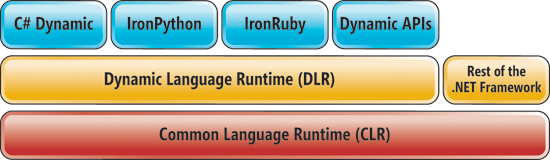
\includegraphics[width=6cm]{cs-dlr}

\end{frame}

\begin{frame}[fragile,plain]
\frametitle{动态调度示例}
\begin{lstlisting}
  dynamic d = new MyDynamicObject();
  d.Bar("Baz", 3, d);
\end{lstlisting}

\begin{lstlisting}
using System.Dynamic;
class MyDynamicObject : DynamicObject {
  public override bool TryInvokeMember(
                     InvokeMemberBinder binder,
                     object[] args, out object result) {
    Console.WriteLine("Method: {0}", binder.Name);
    foreach (var arg in args)
      Console.WriteLine("Argument: {0}", arg);
    result = args[0];
    return true;
  }
}
\end{lstlisting}

\begin{lstlisting}[language=Clean]
Method: Bar
Argument: Baz
Argument: 3
Argument: MyDynamicObject
\end{lstlisting}
\end{frame}


\begin{frame}[fragile]
\frametitle{可选参数(\textit{Optional Parameters})}
\begin{itemize}
\item 函数定义时给定默认值
\begin{lstlisting}
public void func(int x, int y = 5, int z = 7);
\end{lstlisting}
\item 函数调用时,可以省略有默认值的参数
\begin{lstlisting}[escapeinside=<>]
func(1, 2, 3); // <正常调用>
func(1, 2);    // <省略z, 等价于>func(1, 2, 7)
func(1);       // <省略z, 等价于>func(1, 5, 7)
\end{lstlisting}
\end{itemize}
\end{frame}

\begin{frame}[fragile]
\frametitle{命名参数(\textit{Named Argments})}
\begin{itemize}
\item 参数(\textit{Parameters})名作为名字
\begin{lstlisting}
public void func(int x, int y = 5, int z = 7);
\end{lstlisting}
\item 调用时,通过名字指定值
\begin{lstlisting}[escapeinside=<>]
func(1, z: 3);    // <等价于>func(1,2,3)
func(x: 3, z: 5); // <等价于>func(3,2,5)
func(z: 3, x: 1); // <同上>
\end{lstlisting}
\end{itemize}
\textbf{命名参数}和\textbf{可选参数}简化函数的重载。
\end{frame}

\begin{frame}[fragile]
\frametitle{范型的逆变与协变}
\lstset{emph={Of}}
\begin{lstlisting}[escapeinside='']
IList<string> listStr = new List<string>();
IList<object> listObj = listStr; //'非法转换'
public interface IList<Of T> { ... };
\end{lstlisting}

\begin{lstlisting}[escapeinside='']
// Manager'$\rightarrow$'Employee '(隐式转换)'
IEnumerable<Manager> ms = GetManagers();
IEnumerable<Employee> es = ms;   //'合法转换'
\end{lstlisting}
\begin{itemize}
\item 协变
\lstset{emph={out}}
\begin{lstlisting}
public interface IEnumerable<out T> { /* ... */ }
\end{lstlisting}
\item 逆变
\lstset{emph={in}}
\begin{lstlisting}
public interface IComparable<in T> { 
  bool CompareTo(T other); 
}
\end{lstlisting}
\end{itemize}
\end{frame}

% Local Variables:
% mode: LaTeX
% TeX-master: "part-03.tex"
% TeX-header-end: "% End-of-Header$"
% TeX-trailer-start: "% Start-of-Trailer$"
% coding: utf-8
% End:

